% !TEX TS-program = xelatex
% !TEX encoding = UTF-8
\documentclass{WMUDoctor}
\graphicspath{{figures/}}
\begin{document}
    %=====封皮页需要自己填写的内容
    % 标题样式 使用 \title{{}}; 使用时必须保证至少两个外侧括号
    %  如:短标题 \title{{第一行}},
    %     长标题 \title{{第一行}{第二行}}
    %     超长标题\tiitle{{第一行}{...}{第N行}}
    \title{{温州医科大学博士示例论文}}%中文标题
    \entitle{{Doctor's Thesis Template of Wenzhou Medical Unviersity}}%英文标题
    %\chair{赵XX教授\ \ 温州医科大学}
    %\chair{{赵XX教授}, {温州医科大学}}
    % \chair{赵XX}{教授}{温州医科大学}
    %\member{{XX教授 温州医科大学}{XX教授 温州医科大学}{XX教授 温州医科大学}{XX教授 温州医科大学}{XX教授 温州医科大学}}
    \categoryid{R5}%论文分类
    \codeid{10343}%单位代码
    \studentid{18200XXXX}%学号
    \author{Angus Zhang}%论文作者
    \major{重症医学}%专业、年级
    \studytype{学术型}%培养类型
    \advisor{潘老师}%指导老师
    \submityear{二〇}%提交年份二〇二〇就填二〇
    \submitmonth{六}%提交月份
    %%======生成封面(几乎不需要更改)
    \maketitle
    \frontmatter
    %======生成目录
    \tableofcontents
    %======插图索引和附表索引
    \renewcommand{\listfigurename}{插图索引}
    \renewcommand{\listtablename}{附表索引}
    \setcounter{lofdepth}{1}
    \newcommand{\loflabel}{图~}
    \renewcommand{\numberline}[1]{\songti\zihao{4}\loflabel~#1\hspace*{\baselineskip}}
    \addcontentsline{toc}{chapter}{插图索引}
    \listoffigures
    \newcommand{\lotlabel}{表~}
    \renewcommand{\numberline}[1]{\songti\zihao{4}\lotlabel~#1\hspace*{\baselineskip}}
    \addcontentsline{toc}{chapter}{附表索引}
    \listoftables
    %% !TEX encoding = UTF-8
%======中文摘要内容格式:{中文摘要}{关键词}
\ZhAbstract{我是目的。}{我是方法。}{我是结果。}{我是结论。}{温州医科大学;浙江省重点建设高校}
%======中文摘要内容格式:{英文摘要}{关键词}
\EnAbstract{I'm Objective.}{I'm Methods.}{I'm Results.}{I'm Conclusions.}{WMU, Priority Development University of Zhejiang Province}%学校模板貌似把摘要和正文一起编页码了,所以这个部分挪到了后面
    %======文章主体
    \mainmatter                                                                                                                                                                                                                                                      
    % !TEX encoding = UTF-8
%======中文摘要内容格式:{中文摘要}{关键词}
\ZhAbstract{我是目的。}{我是方法。}{我是结果。}{我是结论。}{温州医科大学;浙江省重点建设高校}
%======中文摘要内容格式:{英文摘要}{关键词}
\EnAbstract{I'm Objective.}{I'm Methods.}{I'm Results.}{I'm Conclusions.}{WMU, Priority Development University of Zhejiang Province}%如果中英文摘要和目录一起罗马数字编页码,请把部分移到\mainmatter前
    % !TEX encoding = UTF-8
\chapter{前~~~~言}
% \Preface{}
\section{Why \LaTeX ? }
\LaTeX{} ,是一种基于\TeX{}的排版系统,由美国计算机科学家莱斯利·兰伯特在20世纪80年代初期开发,利用这种格式系统的处理,即使用户没有排版和程序设计的知识也可以充分发挥由\TeX{}所提供的强大功能,不必一一亲自去设计或校对,能在几天,甚至几小时内生成很多具有书籍质量的印刷品。对于生成复杂表格和数学公式,这一点表现得尤为突出。因此它非常适用于生成高印刷质量的科技和数学、物理文档。这个系统同样适用于生成从简单的信件到完整书籍的所有其他种类的文档。

为了方便温州医科大学将更多的时间集中于论文的内容当中,而不是在格式的调节上浪费时间。\LaTeX{} 提供了一个很好的方式。\LaTeX{} 的优点很多,多的像天上的星星数不清,我就不一一列举了,大家可以多用用。有什么问题联系请提交GitHub的issue,能解答一定解答。
\par 下文,与温医大研〔2013〕23号文件《温州医科大学研究生学位论文编排及打印格式要求》中要求一致。若有不同请与我联系。

\clearpage%各个章节内容单独分开撰写,方便编译和组织;
    % !TEX encoding = UTF-8
\chapter{材料与方法}
% \Method

正确编译需要以下几个部分(这是一个列表环境):
\begin{itemize}
    \item 一个基本的\TeX{}发行版
    \item CJK或XeCJK(供\LaTeX{})宏包
    \item ctex宏包(提供ctexbook文档).
    \item 中文字体
    \item 如果要使用 biblatex 进行文献列表和引用的排版的话, 还需要 biblatex 宏包。
\end{itemize}

\section{模板使用}
\subsection{模板文件结构\label{sec:files}}
整个模板根目录的文件列表如下:
\begin{center}
    \begin{tabular}{llc}
        \toprule
        文件                     & 说明                   & 备注                 \\
        \midrule
        WMUDoctor.cls            & WMUDoctor宏包          & \textcolor{red}{{*}} \\
        WMU.cfg                  & WMU宏包配置文件        & \textcolor{red}{{*}} \\
        WMUbib.bst               & 引文样式文件           & \textcolor{red}{{*}} \\
        references/reference.bib & bib数据库              & \textcolor{red}{{*}} \\
        figures/wmu.jpg          & 温州医科大学校名标准字 & \textcolor{red}{{*}} \\
        WMUBachelorTemplate.tex  & \TeX{}样例文件         & \textcolor{red}{{*}} \\
        \bottomrule
    \end{tabular}
\end{center}
注: \textcolor{red}{{*}} 表示\LaTeX{}模板必须的文件。
\subsection{示例}
对于论文中最常使用的一些功能在本节中给出示例。
\subsection{公式}
\begin{equation}
    \hat{H}=\frac{\epsilon}{2}\hat{\sigma}_{z}-\frac{\Delta}{2}\hat{\sigma}_{x}+\sum_{k}\omega_{k}\hat{b}_{k}^{\dagger}\hat{b}_{k}+\sum_{k}\frac{g_{k}}{2}\hat{\sigma}_{z}(\hat{b}_{k}+\hat{b}_{k}^{\dagger})\label{eq:sbm}
\end{equation}

根据公式\ref{eq:sbm}可知,这个是对公示的引用。
\begin{align}\label{eqn3:9}
    \int_{-\infty}^{+\infty}S(\tau,f)\,\mathrm{d}\tau & =\int_{-\infty}^{+\infty}x(t)\left\{\int_{-\infty}^{+\infty}\frac{|f|}{\sqrt{2\pi}}e^{\frac{-|f|^2(\tau-t)^2}{2}}\,\mathrm{d}\tau\right\}e^{-j2\pi ft}\,\mathrm{d}t\notag                                  \\
                                                      & =\int_{-\infty}^{+\infty}x(t)e^{-j2\pi ft}\left\{\int_{-\infty}^{+\infty}\frac{1}{\sqrt{\pi}}e^{-\left[\frac{|f|(\tau-t)}{\sqrt{2}}\right]^2}\,\mathrm{d}\frac{|f|(\tau-t)}{\sqrt{2}}\right\}\,\mathrm{d}t
\end{align}
令$\theta=\frac{|f|(\tau-t)}{\sqrt{2}}$,则式\eqref{eqn3:9}可改写为
\begin{align}\label{eqn3:10}
    \int_{-\infty}^{+\infty}S(\tau,f)\,\mathrm{d}\tau & =\int_{-\infty}^{+\infty}x(t)e^{-j2\pi ft}\,\mathrm{d}t\frac{1}{\sqrt{\pi}}\int_{-\infty}^{+\infty}e^{-\theta^2}\,\mathrm{d}\theta\notag \\
                                                      & =\int_{-\infty}^{+\infty}x(t)e^{-j2\pi ft}\,\mathrm{d}t\frac{2}{\sqrt{\pi}}\int_{0}^{+\infty}e^{-\theta^2}\,\mathrm{d}\theta\notag       \\
                                                      & =\int_{-\infty}^{+\infty}x(t)e^{-j2\pi ft}\,\mathrm{d}t\notag                                                                            \\
                                                      & =X(f)
\end{align}
\subsection{表格}
\begin{table}[H]
    \begin{center}
        \caption{希腊字母表\label{tab:Greek}}
        \begin{tabular}{ccccc}
            \toprule[1.5pt]
            Alpha    & Beta    & Gamma    & Delta    & Theta    \\
            \midrule[0.75pt]
            $\alpha$ & $\beta$ & $\gamma$ & $\delta$ & $\theta$ \\
            $A$      & $B$     & $\Gamma$ & $\Delta$ & $\Theta$ \\
            \bottomrule[1.5pt]
        \end{tabular}
    \end{center}
\end{table}
这是对表\ref{tab:Greek}的引用

\begin{table}[htbp]
    \caption{不同电力系统频率测量算法时间复杂度比较}\label{table2:1}
    \vspace{0.5em}\centering\zihao{5}
    \begin{tabular}{cccc}
        \toprule[1.5pt]
        算法     & 加法                  & 乘法                      & 时间复杂度    \\
        \midrule[0.75pt]
        TQDS     & $QN^2+QN/2+Q+1$       & $QN^2$                    & $O(N^2)$      \\
        WIFFT    & $(QN+1)\log_2(QN+1)$  & $(QN+1)*(1+\log_2(QN+1))$ & $O(N\log_2N)$ \\
        本章算法 & $3(QN+1)\log_2(QN+1)$ & $(QN+1)(1+3\log_2(QN+1))$ & $O(N\log_2N)$ \\
        \bottomrule[1.5pt]
    \end{tabular}
    \vspace{\baselineskip}
\end{table}

本章对时域准同步算法(Time Domain Quasi-synchronous,TQDS)、加窗插值~FFT~算法(Windowed Interpolated FFT,WIFFT)以及本章所提算法的时间复杂度进行分析。因~TQDS~需要进行迭代运算,故设总采样点数为~$QN+1$,其中~$Q$~为迭代次数,$N$~为单次迭代所需的数据点长度。TQDS~共需要~$QN^2$~次加法和~$QN^2+QN/2+Q+1$~次乘法,因此~TQDS~的时间复杂度为~$O(N^2)$。WIFFT~的计算量主要为~FFT~运算,共需进行~$(QN+1)\log_2(QN+1)$~次加法和~$(QN+1)(1+\log_2(QN+1))$~次乘法,因此~WIFFT~的时间复杂度为~$O(N\log_2N)$。对于本章所提出的算法,由于线性卷积运算采用快速卷积来进行计算,因此共需进行~$3(QN+1)\log_2(QN+1)$~加法和~$(QN+1)(1+3\log_2(QN+1))$~次乘法,算法时间复杂度为~$O(N\log_2N)$。表~\ref{table2:1}~对三种频率测量算法的时间复杂度进行了对比。由表~\ref{table2:1}~可见,TQDS~的时间复杂度比其它两种算法要高,本章算法和~WIFFT~时间复杂度相当,有利于算法的实时实现。
\subsection{图形}
这个示例为插入图片:
\begin{figure}[H]
    \centering
    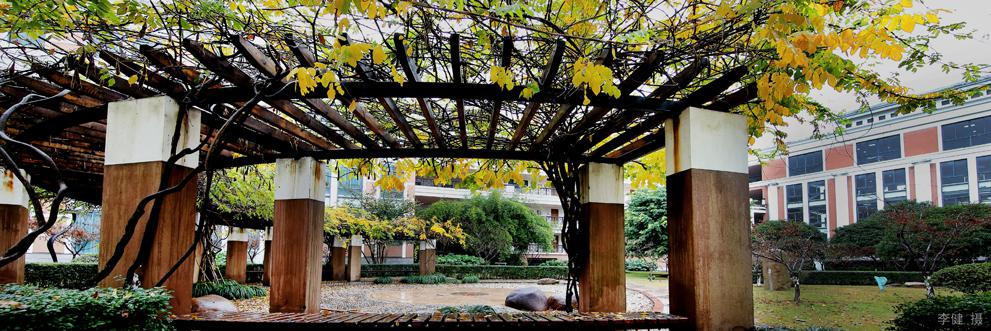
\includegraphics[width=0.8\textwidth]{f1.jpg}%图片名称,放在/figures目录下
    \caption{图片插入\label{fig:fig}}
\end{figure}

具体代码:
\begin{verbatim}
%抄写环境
\begin{figure}[H]
\centering
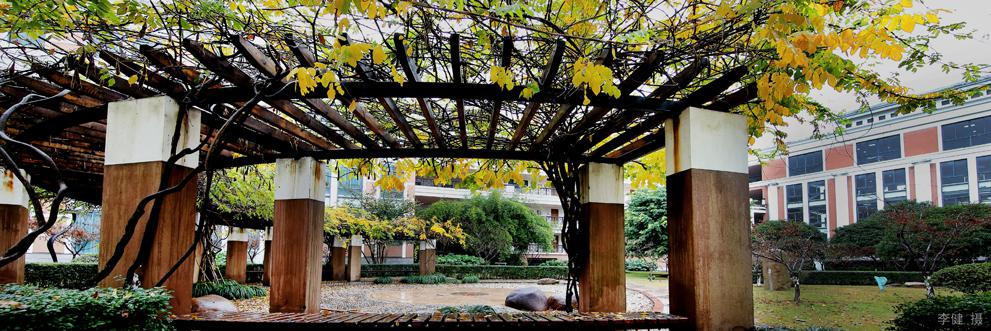
\includegraphics[width=0.8\textwidth]{f1.jpg}%图片放在/figures目录下
\caption{图片插入\label{fig:fig}}
\end{figure}
\end{verbatim}
\begin{figure}[H]
    \centering
    \includegraphics[width=0.8\textwidth]{WMU.jpg}
    \caption{温州医科大学题字及LOGO\label{fig:WMU}}
\end{figure}
对于图\ref{fig:fig}和图\ref{fig:WMU}的引用。


\subsection{引用}
\subsubsection{交叉引用}
对所有需要引用的公式、表格、图形,执行插入--标签后,即可使用插入-- 交叉引用自动产生引用。
\begin{itemize}
    \item 哈密顿量见方程~\eqref{eq:sbm}。
    \item 希腊字母表见表~\ref{tab:Greek}。引用格式与方程引用格式不同
    \item 校名标准字如图~\ref{fig:WMU}。 引用格式与方程引用格式不同
\end{itemize}
具体见代码:
\begin{verbatim}
\begin{itemize}
\item 哈密顿量见方程~\eqref{eq:sbm}。
\item 希腊字母表见表~\ref{tab:Greek}。引用格式与方程引用格式不同
\item 校名标准字如图~\ref{fig:WMU}。 引用格式与方程引用格式不同
\end{itemize}
\end{verbatim}

\subsubsection{文献引用}
将引文的bib数据库(默认文件名为reference.bib)放入模板根目录下的references文件夹,即可通过插入--文献引用自动产生引文。
\begin{itemize}
    \item Journal:An article \upcite{ELIDRISSI94,MELLINGER96,SHELL02,cnarticle}。
    \item Book:An book \cite{IEEE-1363,tex,companion}。
    \item Conference:A conference \cite{kocher99,DPMG,cnproceed}。
    \item Manual:A manual\cite{NPB2}.
    \item MasterThesis:\cite{zhubajie,metamori2004,shaheshang,FistSystem01}.
\end{itemize}
\section{伪代码实现}
\begin{algorithm}
    \caption{放进冰箱的大象}\label{算法实例}
    \begin{algorithmic}
        \REQUIRE 有一只大象
        \ENSURE 放进冰箱里
        \FOR {没有剩余的大象}
        \IF {大象比冰箱大}
        \STATE 把大象分割
        \ENDIF
        \ENDFOR
        \STATE 第一步
        \STATE 第二步
        \STATE 第三步
    \end{algorithmic}
    AAA\end{algorithm}
\subsection{代码展示}
可以把你的程序添加到附录里,展示自己的工作。
\begin{lstlisting}[language={[ANSI]C}, numbers=left]
#include <stdio.h>
int main(int argc, char ** argv)
{
/*打印Hello,world*/
printf("Hello, world!\n");

return 0;
}
\end{lstlisting}
\section{依赖}
WMUDoctor依赖于以下宏包,这些宏包在常见的\LaTeX{}发行版中都包括,在安装使用之前,请确定你的\TeX{}发行版中都已正常安装这些宏包
\begin{table}[H]
    \centering
    \begin{tabular}{cccc}
        \toprule
        \multicolumn{4}{c}{依赖宏包} \\
        \midrule
        {footmisc}    & {amsmath}  & {amsfonts} & {amssymb}   \\
        
        {graphicx}    & {svgnames} & {xcolor}   & {mathptmx}  \\

        {float}       & {fontenc}  & {fancyhdr} & {lastpage}  \\

        {etoolbox}    & {fancy}    & {caption}  & {array}     \\

        {makecell}    & {forloop}  & {xstring}  & {hyperref}  \\

        {tabularx}    & {enumitem} & {ntheorem} & {algorithm} \\

        {algorithmic} & {bibentry} & {xeCJK}    & {CJK}       \\
        {listings}    & {courier}  & {}         & {}          \\
        \bottomrule
    \end{tabular}
\end{table}
如果你尚未安装这些宏包,可以启动你的 \TeX{} 发行版的宏包管理器
来安装;或者到 \url{http://www.ctan.org} 上搜索下载并安装。

\section{基本设置}

\begin{enumerate}[label=(\arabic*)]
    \item 图片搜索路径默认设置为模板根目录下的figures/。
    \item bib数据库默认设置为模板根目录下的references/reference.bib。其中bib文件可由任意文献库管理软件自动生成。
\end{enumerate}

% 简单帮助
\section{文字命令}
\LaTeX 提供了一系列命令,用于修改字体、字号、数字等的呈现形式。

本论文中字体如下:
\subsection{字体}
\begin{verbatim}
宋体: \songti    启用宋体。
黑体: \heiti     启用黑体。
仿宋: \fangsong  启用仿宋。
楷书: \kaishu    启用楷书。
\end{verbatim}
{\songti 宋体} {\heiti 黑体}    {\fangsong 仿宋}     {\kaishu 楷书}

\subsection{字形}
\begin{verbatim}
粗体BOLD:  \textbf{粗体BOLD} 启用粗体
斜体ITALIC:\textbf{粗体BOLD} 启用斜体
\end{verbatim}
{\textbf{粗体BOLD}} {\textit{斜体ITALIC}}

\subsection{字号}%
\begin{center}
	\begin{tabular}{cccccccc}
		\toprule
		初号 & 小初 & 一号 & 小一 & 二号 & 小二 & 三号 & 小三 \\
		0 & -0 & 1 & -1 & 2 & -2 & 3 & -3 \\
		\hline
		四号 & 小四 & 五号 & 小五 & 六号 & 小六 & 七号 & 八号 \\
		4 & -4 & 5 & -5 & 6 & -6 & 7 & 8 \\
		\bottomrule
	\end{tabular}
\end{center}
{\zihao{0}初号}; \dots {\zihao{4}四号};\dots {\zihao{7}{七号}}

\subsection{划线标记}
\begin{verbatim}
下划线:    \uline{下划线}      启用下划线
双下划线:  \uuline{双下划线}   启用双下划线
波浪线:    \uwave{波浪线}      启用波浪线
删除线:    \sout{删除线}       启用删除线
斜删除线:  \xout{斜删除线}     启用斜删除线
\end{verbatim}
{\uline{下划线}} {\uuline{双下划线}} {\uwave{波浪线}} {\sout{删除线}} {\xout{斜删除线}}

\clearpage

    % !TEX encoding = UTF-8
\chapter{系统配置}
正确编译需要以下几个部分(这是一个列表环境):
\begin{itemize}
\item 一个基本的TEX发行版
\item CJK或XeCJK(供\LaTeX{})宏包
\item ctex宏包(提供ctexbook文档).
\item 中文字体
\item 如果要使用 biblatex 进行文献列表和引用的排版的话, 还需要 biblatex 宏包。
\end{itemize}
    % !TEX encoding = UTF-8
\chapter{模板使用}
\section{模板文件结构\label{sec:files}}
整个模板根目录的文件列表如下:
\begin{center}
\begin{tabular}{|l|l|l|}
\hline
WMUDoctor.cls & ---WMUDoctor宏包 & \textcolor{red}{{*}}\\
\hline
WMU.cfg & ---WMU宏包配置文件 & \textcolor{red}{{*}}\\
\hline
WMUbib.bst & ---引文样式文件 & \textcolor{red}{{*}}\\
\hline
references/reference.bib & ---bib数据库 & \textcolor{red}{{*}}\\
\hline
figures/WMU.bmp & ---湖南师范大学大学校名标准字 & \textcolor{red}{{*}}\\
\hline
WMUBachelorTemplate.tex & ---\TeX{}样例文件 &\textcolor{red}{{*}}\\
\hline
\end{tabular}
\end{center}
注: \textcolor{red}{{*}} 表示\LaTeX{}模板必须的文件。
\section{示例}
对于论文中最常使用的一些功能在本节中给出示例。
\subsection{公式}
\begin{equation}
\hat{H}=\frac{\epsilon}{2}\hat{\sigma}_{z}-\frac{\Delta}{2}\hat{\sigma}_{x}+\sum_{k}\omega_{k}\hat{b}_{k}^{\dagger}\hat{b}_{k}+\sum_{k}\frac{g_{k}}{2}\hat{\sigma}_{z}(\hat{b}_{k}+\hat{b}_{k}^{\dagger})\label{eq:sbm}
\end{equation}
根据公式\ref{eq:sbm}可知,这个是对公示的引用。
\begin{align}\label{eqn3:9}
\int_{-\infty}^{+\infty}S(\tau,f)\,\mathrm{d}\tau&=\int_{-\infty}^{+\infty}x(t)\left\{\int_{-\infty}^{+\infty}\frac{|f|}{\sqrt{2\pi}}e^{\frac{-|f|^2(\tau-t)^2}{2}}\,\mathrm{d}\tau\right\}e^{-j2\pi ft}\,\mathrm{d}t\notag\\
&=\int_{-\infty}^{+\infty}x(t)e^{-j2\pi ft}\left\{\int_{-\infty}^{+\infty}\frac{1}{\sqrt{\pi}}e^{-\left[\frac{|f|(\tau-t)}{\sqrt{2}}\right]^2}\,\mathrm{d}\frac{|f|(\tau-t)}{\sqrt{2}}\right\}\,\mathrm{d}t
\end{align}
令$\theta=\frac{|f|(\tau-t)}{\sqrt{2}}$,则式\eqref{eqn3:9}可改写为
\begin{align}\label{eqn3:10}
\int_{-\infty}^{+\infty}S(\tau,f)\,\mathrm{d}\tau&=\int_{-\infty}^{+\infty}x(t)e^{-j2\pi ft}\,\mathrm{d}t\frac{1}{\sqrt{\pi}}\int_{-\infty}^{+\infty}e^{-\theta^2}\,\mathrm{d}\theta\notag\\
&=\int_{-\infty}^{+\infty}x(t)e^{-j2\pi ft}\,\mathrm{d}t\frac{2}{\sqrt{\pi}}\int_{0}^{+\infty}e^{-\theta^2}\,\mathrm{d}\theta\notag\\
&=\int_{-\infty}^{+\infty}x(t)e^{-j2\pi ft}\,\mathrm{d}t\notag\\
&=X(f)
\end{align}
\subsection{表格}
\begin{table}[H]
	\begin{center}
		\caption{希腊字母表\label{tab:Greek}}
		\begin{tabular}{|c|c|c|c|c|}
			\hline
			Alpha & Beta & Gamma & Delta & Theta\\
			\hline
			$\alpha$ & $\beta$ & $\gamma$ & $\delta$ & $\theta$\\
			\hline
			$A$ & $B$ & $\Gamma$ & $\Delta$ & $\Theta$\\
			\hline
		\end{tabular}
		\end{center}
\end{table}
这是对表\ref{tab:Greek}的引用

\begin{table}[htbp]
	\caption{不同电力系统频率测量算法时间复杂度比较}\label{table2:1}
	\vspace{0.5em}\centering\zihao{5}
	\begin{tabular}{cccc}
		\toprule[1.5pt]
		算法 &  加法 & 乘法 & 时间复杂度 \\
		\midrule[1pt]
		TQDS       & $QN^2+QN/2+Q+1$        &$QN^2$                      & $O(N^2)$     \\
		WIFFT         & $(QN+1)\log_2(QN+1)$ & $(QN+1)*(1+\log_2(QN+1))$ &$O(N\log_2N)$\\
		本章算法 &$3(QN+1)\log_2(QN+1)$    & $(QN+1)(1+3\log_2(QN+1))$          & $O(N\log_2N)$\\
		\bottomrule[1.5pt]
	\end{tabular}
	\vspace{\baselineskip}
\end{table}

本章对时域准同步算法(Time Domain Quasi-synchronous,TQDS)、加窗插值~FFT~算法(Windowed Interpolated FFT,WIFFT)以及本章所提算法的时间复杂度进行分析。因~TQDS~需要进行迭代运算,故设总采样点数为~$QN+1$,其中~$Q$~为迭代次数,$N$~为单次迭代所需的数据点长度。TQDS~共需要~$QN^2$~次加法和~$QN^2+QN/2+Q+1$~次乘法,因此~TQDS~的时间复杂度为~$O(N^2)$。WIFFT~的计算量主要为~FFT~运算,共需进行~$(QN+1)\log_2(QN+1)$~次加法和~$(QN+1)(1+\log_2(QN+1))$~次乘法,因此~WIFFT~的时间复杂度为~$O(N\log_2N)$。对于本章所提出的算法,由于线性卷积运算采用快速卷积来进行计算,因此共需进行~$3(QN+1)\log_2(QN+1)$~加法和~$(QN+1)(1+3\log_2(QN+1))$~次乘法,算法时间复杂度为~$O(N\log_2N)$。表~\ref{table2:1}~对三种频率测量算法的时间复杂度进行了对比。由表~\ref{table2:1}~可见,TQDS~的时间复杂度比其它两种算法要高,本章算法和~WIFFT~时间复杂度相当,有利于算法的实时实现。
\subsection{图形}
这个示例为插入图片:
\begin{figure}[H]
	\centering
		
\includegraphics[width=0.618\textwidth]{figure.jpg}%图片名称,放在/figures目录下
	\caption{图片插入\label{fig:fig}}
\end{figure}
具体代码:
\begin{verbatim}%抄写环境
\begin{figure}[H]
\centering

\includegraphics[width=0.618\textwidth]{figure.jpg}%图片放在/figures目录下
\caption{图片插入\label{fig:fig}}
\end{figure}
\end{verbatim}
\begin{figure}[H]
\centering
		\includegraphics[width=0.618\textwidth]{WMU.jpg}
\caption{湖南师范大新大学校名标准字\label{fig:WMU}}
\end{figure}
对于图\ref{fig:fig}和图\ref{fig:WMU}的引用。
\subsection{引用}
\subsubsection{交叉引用}
对所有需要引用的公式、表格、图形,执行插入--标签后,即可使用插入-- 交叉引用自动产生引用。
\begin{itemize}
\item 哈密顿量见方程~\eqref{eq:sbm}。
\item 希腊字母表见表~\ref{tab:Greek}。引用格式与方程引用格式不同
\item 校名标准字如图~\ref{fig:WMU}。 引用格式与方程引用格式不同
\end{itemize}
具体见代码:
\begin{verbatim}
\begin{itemize}
\item 哈密顿量见方程~\eqref{eq:sbm}。
\item 希腊字母表见表~\ref{tab:Greek}。引用格式与方程引用格式不同
\item 校名标准字如图~\ref{fig:WMU}。 引用格式与方程引用格式不同
\end{itemize}
\end{verbatim}
\subsubsection{文献引用}
将引文的bib数据库(默认文件名为reference.bib)放入模板根目录下的references文件夹,即可通过插入--文献引用自动产生引文。
\begin{itemize}
\item Journal:An article \upcite{ELIDRISSI94,MELLINGER96,SHELL02,cnarticle}。
\item Book:An book \cite{IEEE-1363,tex,companion}。
\item Conference:A conference \cite{kocher99,DPMG,cnproceed}。
\item Manual:A manual\cite{NPB2}.
\item MasterThesis:\cite{zhubajie,metamori2004,shaheshang,FistSystem01}.
\end{itemize}
\subsection{伪代码实现}
\begin{algorithm}
\caption{放进冰箱的大象}\label{算法实例}
\begin{algorithmic}
	\REQUIRE 有一只大象
	\ENSURE 放进冰箱里
	\FOR {没有剩余的大象}
	\IF {大象比冰箱大}
	\STATE 把大象分割
	\ENDIF
	\ENDFOR
	\STATE 第一步
	\STATE 第二步
	\STATE 第三步
\end{algorithmic}
AAA\end{algorithm}
\subsection{代码展示}
可以把你的程序添加到附录里,展示自己的工作。
\begin{lstlisting}[language={[ANSI]C}, numbers=left]
#include <stdio.h>
int main(int argc, char ** argv)
{
/*打印Hello,world*/
printf("Hello, world!\n");

return 0;
}
\end{lstlisting}
\section{依赖}
WMUDoctor依赖于以下宏包,这些宏包在常见的\LaTeX{}发行版中都包括,在安装使用之前,请确定你的\TeX{}发行版中都已正常安装这些宏包
\begin{table}[H]
	\centering
	\begin{tabular}{cccc}
		\hline
		{footmisc} &  {amsmath} &  {amsfonts} &  {amssymb} \\
		
		{graphicx} &  {svgnames} &  {xcolor} &  {mathptmx} \\
		
		{float} &  {fontenc} &  {fancyhdr} &  {lastpage} \\
		
		{etoolbox} &  {fancy} &  {caption} &  {array} \\
		
		{makecell} &  {forloop} &  {xstring} &  {hyperref} \\
		
		{tabularx} &  {enumitem} &  {ntheorem} &  {algorithm}\\
		
		{algorithmic} &  {bibentry} &  {xeCJK} &  {CJK} \\
		{listings} &  {courier} &  {} &  {} \\
		\hline
	\end{tabular}
\end{table}
如果你尚未安装这些宏包,可以启动你的 \TeX{} 发行版的宏包管理器
来安装;或者到 \url{http://www.ctan.org} 上搜索下载并安装。
\section{基本设置}
\begin{enumerate}
	\item 图片搜索路径默认设置为模板根目录下的figures/。
	\item bib数据库默认设置为模板根目录下的references/reference.bib。 其中bib文件可由任意文献库管理软件自动生成
\end{enumerate}


    % !TEX encoding = UTF-8
\chapter{小~~~~结}
% \Summary

我是小结。我是小结。我是小结。我是小结。我是小结。

\textit{我是小结。我是小结。我是小结。我是小结。我是小结。}

\textbf{我是小结。我是小结。我是小结。我是小结。我是小结。}

\textbf{\textit{我是小结。我是小结。我是小结。我是小结。我是小结。}}

I'm summaries. I'm summaries. I'm summaries. I'm summaries. I'm summaries.

\textit{I'm summaries. I'm summaries. I'm summaries. I'm summaries. I'm summaries.}

\textbf{I'm summaries. I'm summaries. I'm summaries. I'm summaries. I'm summaries.}

\textbf{\textit{I'm summaries. I'm summaries. I'm summaries. I'm summaries. I'm summaries.}}

\clearpage
    %=======论文后部
    \backmatter
    %=======参考文献1
    % \bibdatabase{references/reference}%参考文献数据库
    \printbib
    % !TEX encoding = UTF-8
\Appendix
这里是附录页,附上你的程序或必要的相关知识

\bf\heiti\color{red}{若要生成目录和参考文献的编译方式:} \color{black}XeLaTeX -->BibTeX --> XeLaTeX--> XeLaTeX%附录
    % !TEX encoding = UTF-8
\chapter{致~~~~谢}

我是致谢。我是致谢。我是致谢。我是致谢。我是致谢。

\textit{我是致谢。我是致谢。我是致谢。我是致谢。我是致谢。}

\textbf{我是致谢。我是致谢。我是致谢。我是致谢。我是致谢。}

\textbf{\textit{我是致谢。我是致谢。我是致谢。我是致谢。我是致谢。}}

I'm thanks. I'm thanks. I'm thanks. I'm thanks. I'm thanks.

\textit{I'm thanks. I'm thanks. I'm thanks. I'm thanks. I'm thanks.}

\textbf{I'm thanks. I'm thanks. I'm thanks. I'm thanks. I'm thanks.}

\textbf{\textit{I'm thanks. I'm thanks. I'm thanks. I'm thanks. I'm thanks.}}

\clearpage%致谢
\end{document}